
\section{Background}\label{sec:background}

\subsection{Voice Acoustics}\label{sec:voice}

The generation of human voice follows a source-filter model~\cite{fant1960acoustic}. A speech signal can be seen as a source signal (the glottal source at the larynx, or noise generated at a constriction in the vocal tract), filtered with the resonances in the cavities of the vocal tract (tongue, teeth, lips, velum, etc. modifying the sound spectrum over time). This theory has been verified using 3-D printed models of two configurations of a vocal tract to generate sounds to generate the vowels in the words ``had'' and ``heard''~\cite{wolfe2016experimentally}. 


A typical adult male will have a fundamental frequency  ($f_0$) of from 85 to 155 Hz, and that of a typical adult female from 165 to 255 Hz~\cite{baken1987clinical,titze1994principles}. The frequencies of the first, second, and the $i$-th resonances are labeled as  $R_1, R_2, \ldots R_i$, and those of the spectral peaks produced by these resonances are called formants, $F_1, F_2, \ldots F_i $~\cite{titze2015toward}. 
%
According to~\cite{ladefoged2014course}, English vowels are perceived largely according to the values of the formants $F_1$ and $F_2$. The range of $F_1$ is roughly from 270 to 860 Hz, and that of $F_2$ from 840 to 2790 Hz~\cite{peterson1952control}. As for English consonants, there are six categories: plosive/stop (e.g. /p/), fricative (e.g. /f/), affricate (e.g. /dZ/), nasal (e.g. /m/), lateral (e.g. /l/), and approximant (e.g. /r/). The frequencies of consonants vary a lot. The turbulence of /s/ and /z/ occurs above 3500Hz, and reaches as high as 10,000 Hz, whereas /w/ has $F_1$ from 250 to 450 Hz and $F_2 $ from 600 to 850 Hz~\cite{ladefoged2012vowels}. 

By Nyquist–Shannon sampling theorem, to properly sample a signal contains no frequency components higher than $f$ Hz, the sampling rate must be at least $2f$ Hz (Nyquist rate). In other words, a sampling rate of 400 Hz (motion sensors' rate as shown in Table~\ref{tab:sample}) can only handle signals whose component frequencies are below 200 Hz. Except for the part of the fundamentals, all $F_1$ and $F_2$ frequencies can not be sensed. Therefore, it is impossible to perceive the signals with such a low sampling rate.
%



%
However, borrowing theories from \textit{compressed sensing}, the {\systemName} system can partially reconstruct the signal and obtain critical information such as the numbers that appeared in a conversation, genders, or even identities of the speakers, etc., from motion sensor readings, as discussed in Section~\ref{sec:threat}.




\begin{figure}[!h]
	\centering
	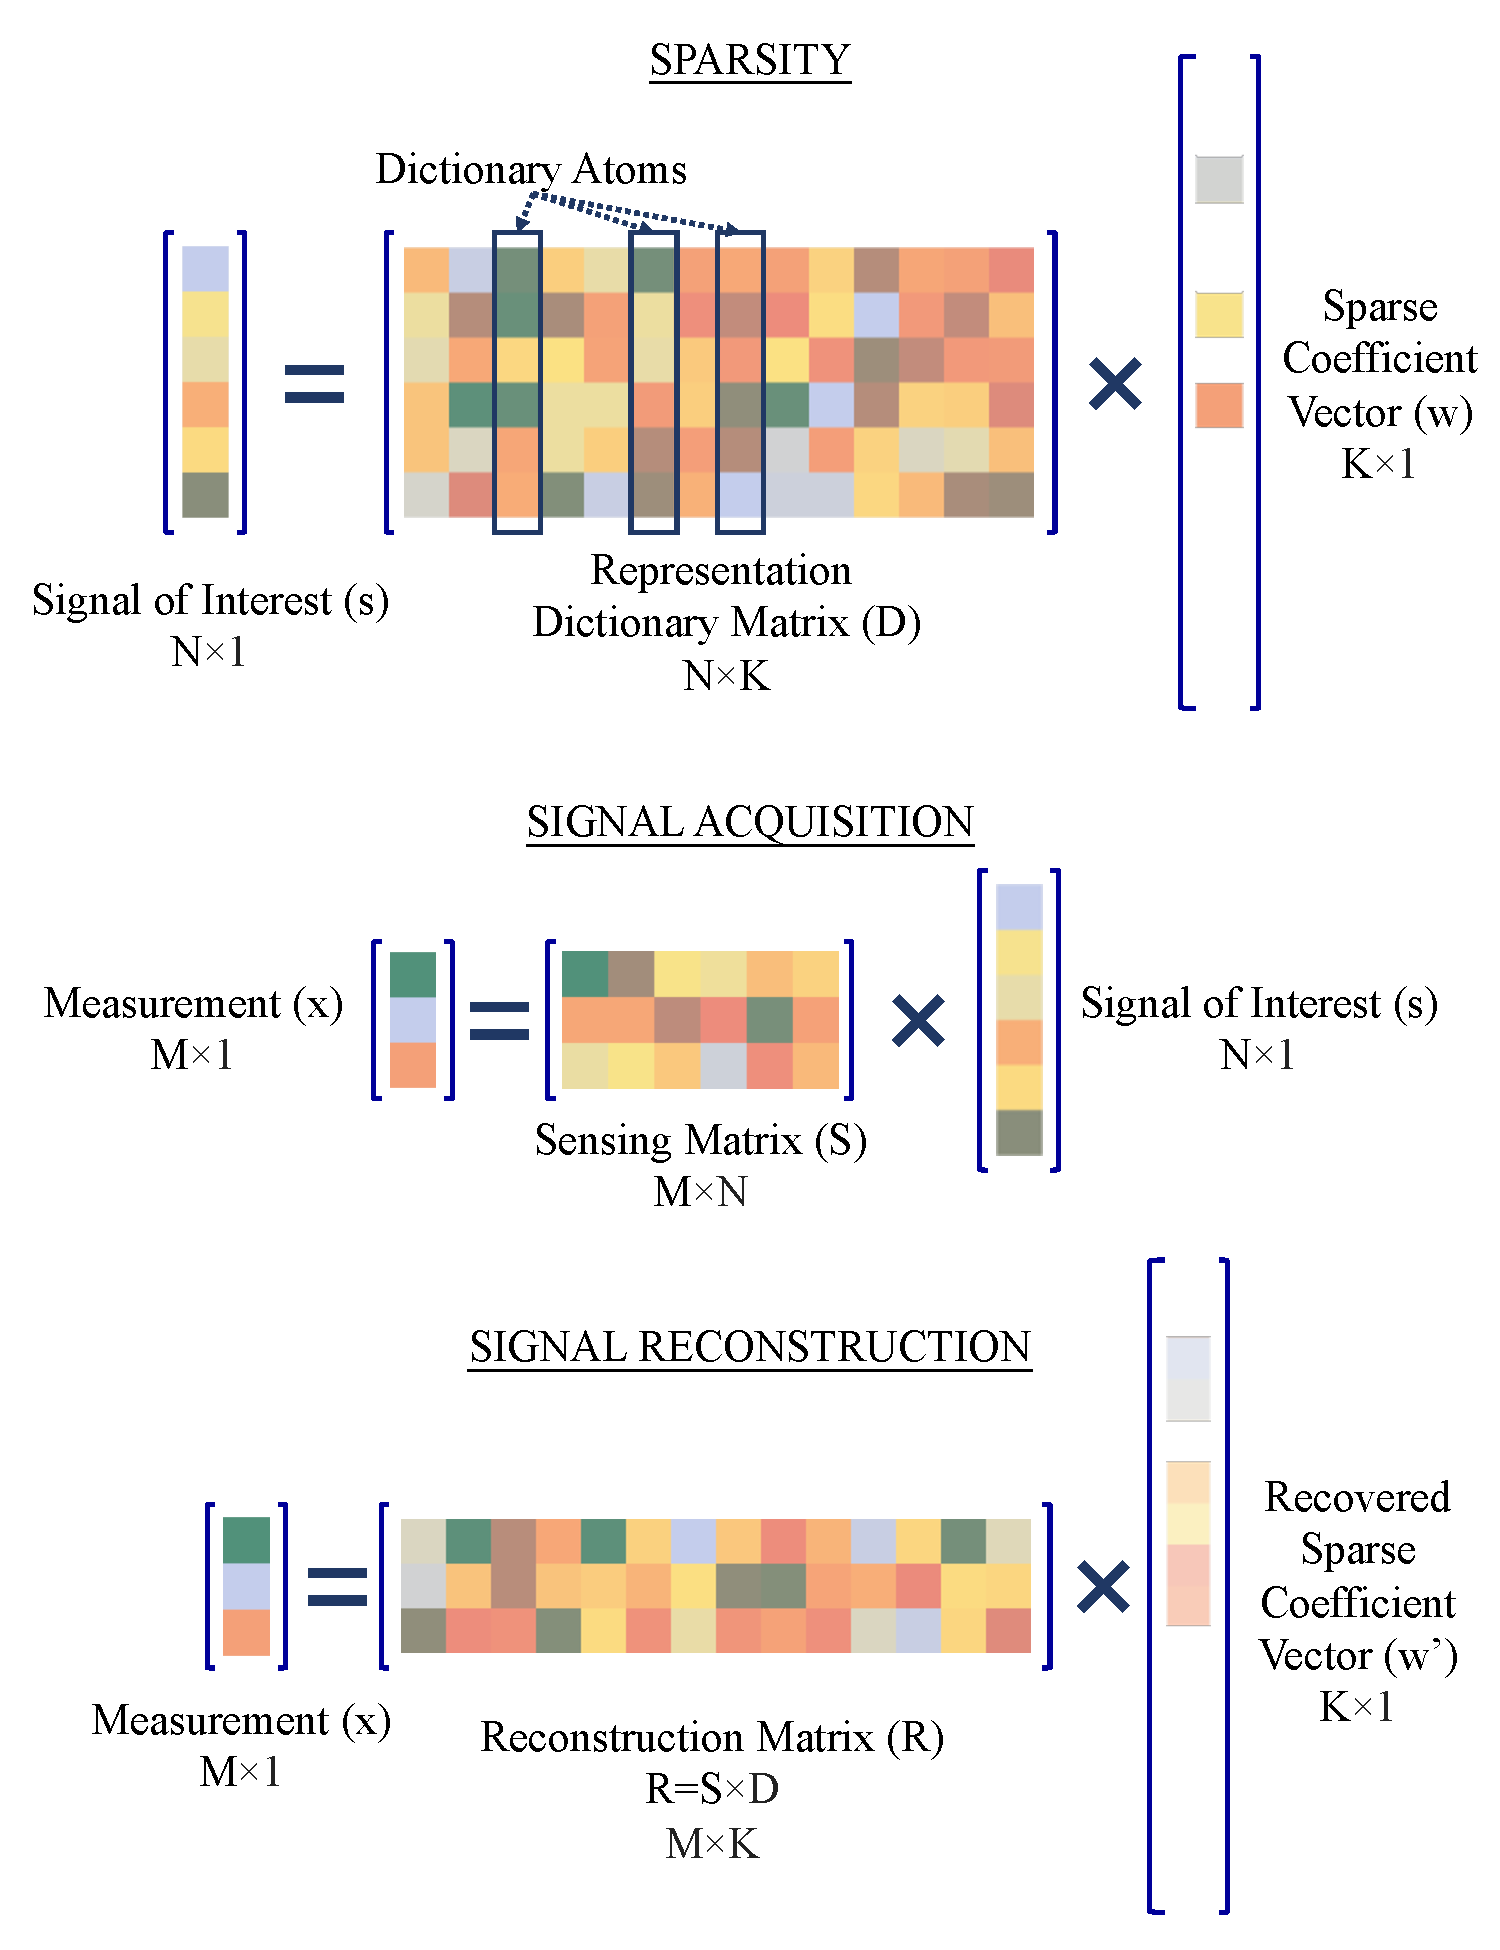
\includegraphics[width=.85\textwidth]{compressed}
	\caption{Mathematical Model of a Typical Compressed Sensing System. }
	\label{fig:compressed}
\end{figure}

\subsection{Compressed Sensing}\label{sec:compressed}

Compressed sensing~\cite{donoho2006compressed} (also known as compressive sensing~\cite{siddamal2015survey}, compressive sampling~\cite{candes2006compressive}) is a novel sensing/sampling paradigm that acquires and reconstructs signals in a much more efficient way than the established Nyquist–Shannon sampling theorem. 


First introduced by Candes et al. in 2004~\cite{candes2004robust}, compressed sensing takes advantage of prior knowledge about inherent characteristics (sparsity) of signals.
In this way, even with far fewer samples, the signal of interest can still be perfectly (or nearly perfectly) recovered. The constraint of the Nyquist rate (sampling rate to be 2 times of signal bandwidth) is no longer a requirement. Therefore, we adopt this technique in the design of the  {\systemName} system.


As shown in Figure~\ref{fig:compressed}, the theory of compressed sensing has solid mathematical backgrounds. 
%
The signals of interest should have a low information rate, i.e., the signal is sparse in its original domain (e.g. time domain) or some transform domain (e.g. frequency domain)~\cite{candes2008introduction}. More precisely, when expressed in a proper representation dictionary $D$, a large number of coefficients in vector $w$ are zeros or small enough to be ignored. In fact, natural signals such as sounds, images,  or seismic data have this sparsity property and can be stored in compressed form, in terms of their projection on a suitable dictionary~\cite{qaisar2013compressive}. 



In the signal acquisition stage, compressed sensing aims to \textit{undersample} the signal of interest such that the dimension size $M$ of measurements $x$ is much smaller than the dimension size $N$ of the signal $s$. This goal is achieved by using a sensing matrix $S$ of size $M \times N$, where $M \ll N$.
%
The reconstruction of the original signal is essentially an optimization problem: 
finding the optimal sparse coefficient vector
$w^\prime_{opt}$ such that 
\begin{equation}\label{eq:reconstruction}
w^\prime_{opt}
=
\argmin_{w^\prime}
\left( 
\gamma
\Vert w^\prime \Vert_p
+
\Vert x - R w^\prime \Vert_2
\right) 
,
\end{equation}
where $\gamma$ is the parameter to balance the evaluation weight of sparsity versus data error, $\Vert w^\prime \Vert_p$ is the $\ell_p$-norm of $w^\prime$, and $R$ is the reconstruction matrix which is equal to $S \times D$. As $\gamma$ increases the solution is getting more sparse. When $p=0$, this optimization problem has been proved to be NP-hard~\cite{natarajan1995sparse}. 


%0-norm (number of non-zeros) the 1-norm (sum of absolute values) or that the error (sum of squared errors) has reached a predefined limit. 





The overall performance of compressed sensing is determined by 3 aspects: how representative is the dictionary, how efficient is the sensing matrix, and how well-performed is optimization solver.
%
There are mainly two types of dictionaries, predefined dictionaries and learned dictionaries. Predefined dictionaries are built from basic functions like Fourier transform. Common dictionaries of this type include the discrete cosine transform basis, wavelet packages, and Gabor bases~\cite{skretting2017sparse}. Learned dictionaries are learned from a training dataset of signals. Methods to build such type of dictionaries include K-SVD~\cite{aharon2006k}, MOD ILS-DLA~\cite{engan2007family}, ODL~\cite{mairal2009online}, RLS-DLA~\cite{skretting2010recursive}, and so on.
%
As for the design of the sensing matrix, it is important to check whether the matrix will allow the recovery of a sparse solution. The most famous one is the restricted isometry property ~\cite{candes2008restricted}, though it has been shown too strict~\cite{donoho2009observed}.
%
The signal reconstruction solvers span a wide series of techniques that include 
greedy pursuit, Bayesian framework, iterative thresholding, convex relaxation, nonconvex optimization, and brute force~\cite{tropp2010computational}. Some well-known solvers include
OMP~\cite{tropp2007signal}, GPSR~\cite{figueiredo2007gradient}, BCS~\cite{ji2008bayesian}, and so on. 
%
More information can be found in survey papers like ~\cite{zhang2015survey,skretting2017sparse,rani2018systematic}.




In our attack design, the audio signals played by smartphone speakers are the signals of interest. When the sound is collected by motion sensors, it is essentially the signal acquisition stage that applies the sensing matrix to get the measurements. The motion data has a very low sampling rate, much lower than the Nyquist rate. However, using a carefully designed reconstruction matrix, the original signals of interest can be (partially) reconstructed from the recovered sparse coefficient vector and the representation dictionary ($s^\prime = D \times w^\prime$).

\subsection{Smartphone Hardware}


\begin{figure}[!h]
	\centering
	\hspace{.25in}
	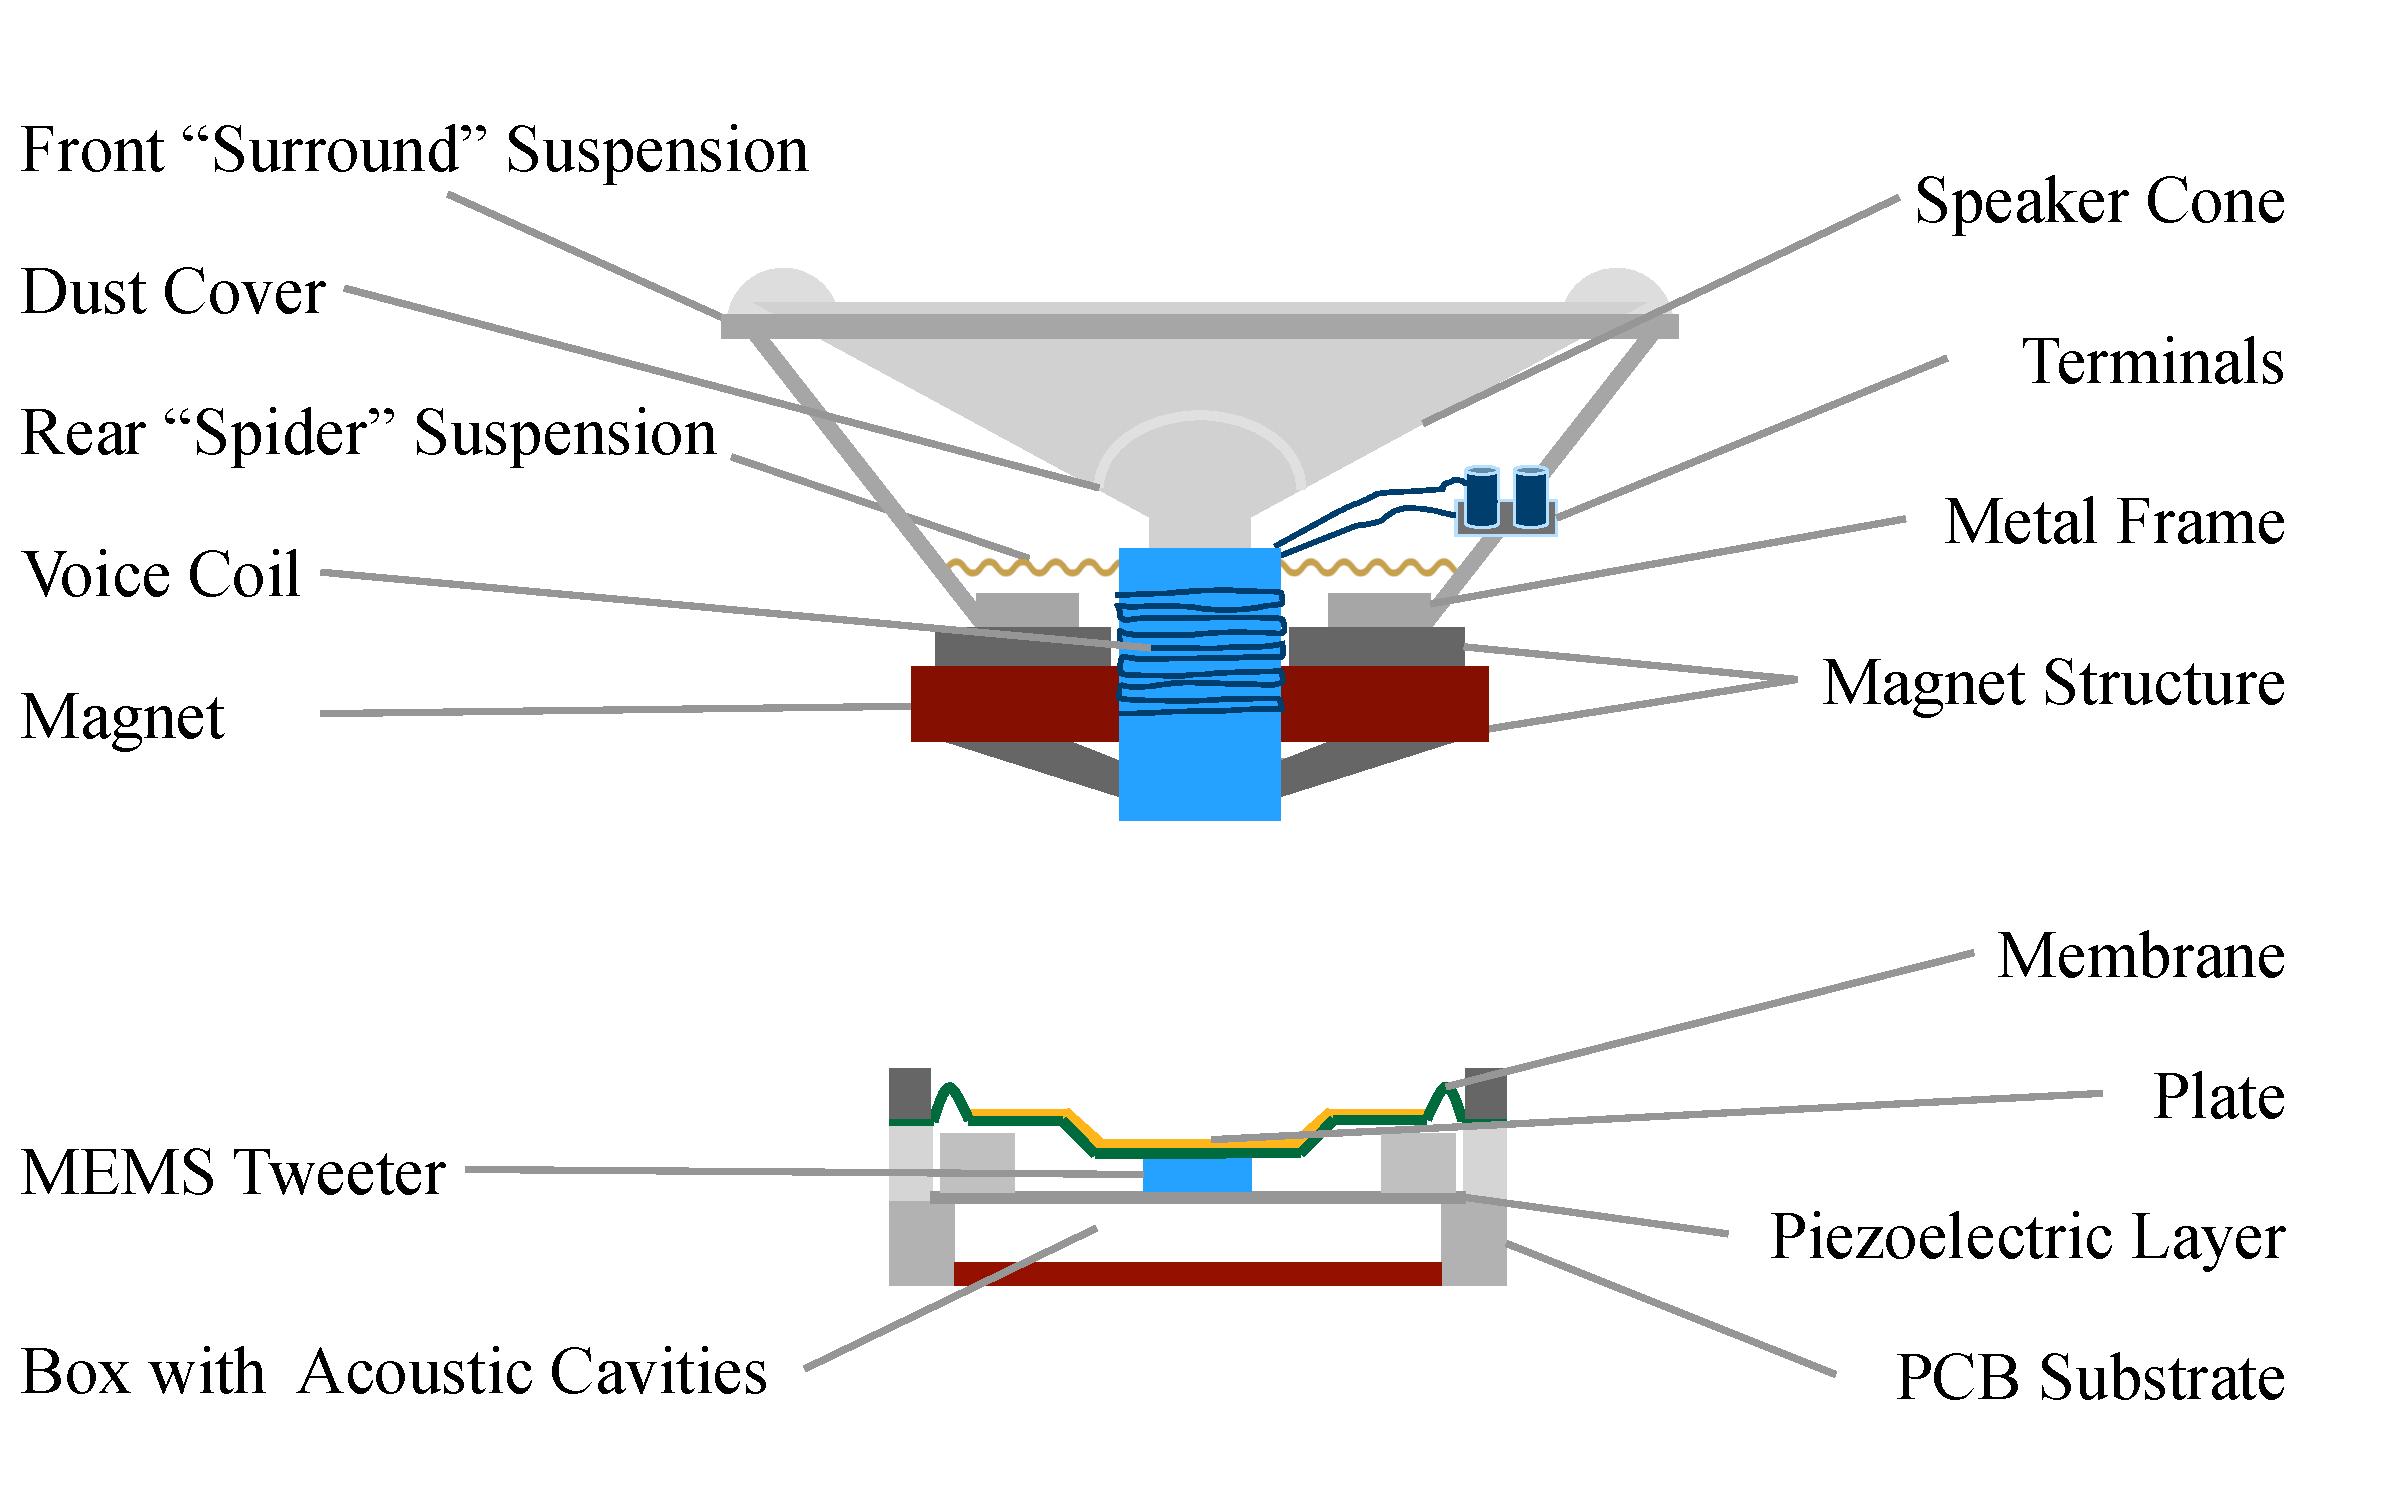
\includegraphics[width=.85\textwidth]{speaker}
	\caption{Structure of a Desktop Loudspeaker Versus a MEMS Speaker.}
	\label{fig:speaker}
\end{figure}

Figure~\ref{fig:speaker} shows the different structures of a typical desktop loudspeaker and a Micro Electro-Mechanical Systems (MEMS) speaker in smartphones. In a desktop loudspeaker, sounds are created by alternating currents to the voice coil, while a smartphone speaker uses a small MEMS tweeter. As a result, the MEMS speaker consumes much less power than the desktop loudspeaker. But for the same reason, the sound pressure level (SPL) generated by MEMS speakers is much lower than that of desktop loudspeakers.



The Google Nexus 6P and Samsung Galaxy S8 used in this work can only generate sound with a maximum output of 78.4~dB
\footnote{\scriptsize \url{https://www.phonearena.com/phones/benchmarks}}. 
The commercial off-the-shelf desktop loudspeaker, the \$22.99 Logitech Multimedia Speakers Z200 as an example, has max SPL greater than 88 dB. 
%
Note that a normal speech between two people typically has a range of 50 to 60 decibels and when they are shouting, the range goes to about 75 dB while 15\% of men can shout over 96 dB~\cite{online2005Voice}.
%
The higher the decibels, the easier for the motion sensors to catch the sound signals. With this respect, performing the {\attackName} attack is harder than Gyrophone~\cite{michalevsky2014gyrophone} or AccelWord~\cite{zhang2015accelword}.

As for the motion sensors, Google Nexus 6P uses Bosch BMI160, whose sampling rate can be 1600 Hz. However, the Android operating system only supports up to 400 Hz in order to save power.





